\documentclass[10pt,a4paper,landscape]{article}

% essential packages
\usepackage[T1]{fontenc}
\usepackage{lmodern}
\usepackage[UKenglish]{babel}
\usepackage{csquotes}
\usepackage{graphicx}
\usepackage{hyperref}
\usepackage{amsmath}
\usepackage{amssymb}
\usepackage{booktabs}
\usepackage{longtable}
\usepackage{xcolor}
\usepackage{listings}
\usepackage{enumitem}
\usepackage[landscape,margin=1.5cm,top=1cm,bottom=1cm]{geometry}
\usepackage{multicol}
\usepackage{fancyhdr}
\usepackage{tcolorbox}
\usepackage{tikz}

% remove page numbering
\pagenumbering{gobble}

% define colors
\definecolor{cpublue}{RGB}{52,152,219}
\definecolor{gpugreen}{RGB}{39,174,96}
\definecolor{centregrey}{RGB}{127,140,141}
\definecolor{lightblue}{RGB}{232,244,248}
\definecolor{lightgreen}{RGB}{232,248,232}
\definecolor{lightgrey}{RGB}{248,248,248}

% spacing
\frenchspacing
\setlength{\parindent}{0pt}
\setlength{\parskip}{0pt}

% custom commands for colored boxes with fixed height
\newtcolorbox{cpubox}{
    colback=lightblue,
    colframe=cpublue,
    boxrule=1.5pt,
    arc=3mm,
    left=8pt,right=8pt,top=8pt,bottom=8pt,
    height=14cm,
    valign=top
}

\newtcolorbox{gpubox}{
    colback=lightgreen,
    colframe=gpugreen,
    boxrule=1.5pt,
    arc=3mm,
    left=8pt,right=8pt,top=8pt,bottom=8pt,
    height=14cm,
    valign=top
}

\newtcolorbox{centrebox}{
    colback=lightgrey,
    colframe=centregrey,
    boxrule=1.5pt,
    arc=3mm,
    left=8pt,right=8pt,top=8pt,bottom=8pt,
    height=14cm,
    valign=top
}

\title{CPU vs GPU: Understanding Parallel Processing}
\author{}
\date{}

\begin{document}

% custom title without maketitle to save space
\begin{center}
{\LARGE \textbf{CPU vs GPU: Understanding Parallel Processing}}
\end{center}

\vspace{5mm}

% three column layout
\begin{minipage}[t]{0.32\textwidth}
\begin{cpubox}
\begin{center}
{\large \textcolor{cpublue}{\textbf{CPU\\The Super Waiter}}}
\end{center}

\vspace{3mm}

% single waiter icon
\begin{center}
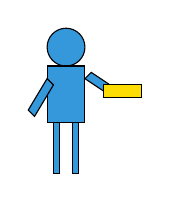
\begin{tikzpicture}[scale=0.8]
% head
\draw[fill=cpublue] (0,1.5) circle (0.3);
% body
\draw[fill=cpublue] (-0.3,1.2) -- (-0.3,0.3) -- (0.3,0.3) -- (0.3,1.2) -- cycle;
% arms
\draw[fill=cpublue] (-0.3,1) -- (-0.6,0.5) -- (-0.5,0.4) -- (-0.2,0.9) -- cycle;
\draw[fill=cpublue] (0.3,1) -- (0.6,0.8) -- (0.7,0.9) -- (0.4,1.1) -- cycle;
% legs
\draw[fill=cpublue] (-0.2,0.3) -- (-0.2,-0.5) -- (-0.1,-0.5) -- (-0.1,0.3) -- cycle;
\draw[fill=cpublue] (0.1,0.3) -- (0.1,-0.5) -- (0.2,-0.5) -- (0.2,0.3) -- cycle;
% tray
\draw[fill=yellow!80!orange] (0.6,0.7) -- (1.2,0.7) -- (1.2,0.9) -- (0.6,0.9) -- cycle;
\end{tikzpicture}
\end{center}

\vspace{3mm}

% feature list
\begin{itemize}[leftmargin=15pt,itemsep=2pt,topsep=0pt]
\item[\textcolor{cpublue}{$>$}] \textbf{4-8 powerful cores}\\
Each highly capable
\item[\textcolor{cpublue}{$>$}] \textbf{Complex tasks}\\
Sequential processing
\item[\textcolor{cpublue}{$>$}] \textbf{Branch prediction}\\
Handles \enquote{if-then} decisions well
\item[\textcolor{cpublue}{$>$}] \textbf{Large cache memory}\\
Quick access to data
\item[\textcolor{cpublue}{$>$}] \textbf{Good for:}\\
Varied tasks, complex decisions
\item[\textcolor{cpublue}{$>$}] \textbf{Example:}\\
Managing restaurant operations
\end{itemize}
\end{cpubox}
\end{minipage}
\hfill
\begin{minipage}[t]{0.32\textwidth}
\begin{centrebox}
\begin{center}
{\large \textcolor{centregrey}{\textbf{Common Ground}}}
\end{center}

\vspace{8mm}

% feature list
\begin{itemize}[leftmargin=15pt,itemsep=2pt,topsep=0pt]
\item[\textcolor{centregrey}{$>$}] \textbf{Team players:}\\
GPU needs CPU to function
\item[\textcolor{centregrey}{$>$}] \textbf{Division of labour:}\\
CPU manages, GPU computes
\item[\textcolor{centregrey}{$>$}] \textbf{Share memory:}\\
Pass data back and forth
\item[\textcolor{centregrey}{$>$}] \textbf{Modern systems:}\\
Use both for best performance
\item[\textcolor{centregrey}{$>$}] \textbf{Like a kitchen:}\\
Manager (CPU) directs workers (GPU)
\end{itemize}
\end{centrebox}
\end{minipage}
\hfill
\begin{minipage}[t]{0.32\textwidth}
\begin{gpubox}
\begin{center}
{\large \textcolor{gpugreen}{\textbf{GPU\\The Army of Waiters}}}
\end{center}

\vspace{3mm}

% multiple waiters icon
\begin{center}
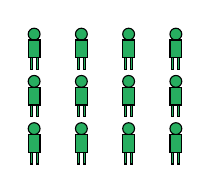
\begin{tikzpicture}[scale=0.5]
% grid of waiters
\foreach \x in {0,1.2,2.4,3.6} {
    \foreach \y in {0,1.2,2.4} {
        % head
        \draw[fill=gpugreen] (\x,\y+0.7) circle (0.15);
        % body
        \draw[fill=gpugreen] (\x-0.15,\y+0.55) rectangle (\x+0.15,\y+0.1);
        % legs
        \draw[fill=gpugreen] (\x-0.1,\y+0.1) rectangle (\x-0.05,\y-0.2);
        \draw[fill=gpugreen] (\x+0.05,\y+0.1) rectangle (\x+0.1,\y-0.2);
    }
}
\end{tikzpicture}
\end{center}

\vspace{3mm}

% feature list
\begin{itemize}[leftmargin=15pt,itemsep=2pt,topsep=0pt]
\item[\textcolor{gpugreen}{$>$}] \textbf{Thousands of simple cores}\\
Modern GPUs: 5,000-10,000+
\item[\textcolor{gpugreen}{$>$}] \textbf{Simple tasks}\\
Massive parallelism
\item[\textcolor{gpugreen}{$>$}] \textbf{Smaller cache per core}\\
But very fast memory access
\item[\textcolor{gpugreen}{$>$}] \textbf{Good for:}\\
Repetitive tasks on lots of data
\item[\textcolor{gpugreen}{$>$}] \textbf{Example:}\\
Serving 1000 identical meals
\end{itemize}
\end{gpubox}
\end{minipage}

\end{document}
